%%%%%%%%%%%%%%%%%%%%%%%%%%%%%%%%%%%%%%%%%%%%%%%%%%%%%%%%%%%%%%%%%%%%%%%%%%%%%%%
\section{Methodology}
\label{sec:methodology}
%%%%%%%%%%%%%%%%%%%%%%%%%%%%%%%%%%%%%%%%%%%%%%%%%%%%%%%%%%%%%%%%%%%%%%%%%%%%%%%

%This paper investigates Monte Carlo as a means to generate multi-group cross sections for fine-mesh transport codes. 

This work required the development of a ``simulation triad'' encompassing three primary simulation tools. First, the OpenMC Monte Carlo code~\citep{romano2013openmc} was utilized to generate multi-group cross sections. Second, the MGXS were used by the OpenMOC code~\citep{boyd2014openmoc} for deterministic multi-group transport calculations. Third, the OpenCG library~\citep{boyd2015opencg} enabled the processing and transfer of tally data on combinatorial geometry (CG) meshes between OpenMC and OpenMOC. Each of the OpenMC, OpenMOC, and OpenCG codes is highlighted in~\autoref{subsec:openmc},~\autoref{subsec:openmoc} and~\autoref{subsec:opencg}.

-outline sections for spatial homogenization?? probably needs further motivating

%In addition, a significant amount of infrastructural code was developed to process the results produced by OpenMC and OpenMOC.


%%%%%%%%%%%%%%%%%%%%%%%%%%%%%%%%%%%%%%%%%%%%%%%%%%%%%%%%%%%%%%%%%%%%%%%%%%%%%%%
\subsection{Continuous Energy Calculations with OpenMC}
\label{subsec:openmc}

The OpenMC continuous energy Monte Carlo (MC) code \citep{romano2013openmc} was employed to generate multi-group cross sections, and reference eigenvalues and pin-wise fission and capture reaction rates. The \texttt{openmc.mgxs} Python module was used to tally multi-group cross sections in CASMO's seventy energy group structure~\citep{rhodes2006casmo} from a single eigenvalue calculation. The multi-group cross sections were calculated with OpenMC's distributed cell tally algorithm~\citep{lax2014distribcell}, which permits spatial tally zones across repeated cell instances. In particular, unique MGXS were computed for each fuel pin cell with distributed cell tallies in the repeating lattice benchmarks described in~\autoref{sec:test-cases}. 

The OpenMC simulations used the ``iso-in-lab'' feature to enforce isotropic in lab scattering. The ``iso-in-lab'' feature samples the outgoing neutron energy from the scattering laws prescribed by the continuous energy cross section library, but the outgoing neutron direction of motion is sampled from an isotropic in lab distribution. Although isotropic in lab scattering is a poor approximation for LWRs, it eliminated scattering source anisotropy as one possible cause of approximation error between OpenMC and OpenMOC. This simplification made it possible to isolate the approximation error resulting from the spatial self-shielding model used to generate MGXS, which is the focal point of this paper.

%%%%%%%%%%%%%%%%%%%%%%%%%%%%%%%%%%%%%%%%%%%%%%%%%%%%%%%%%%%%%%%%%%%%%%%%%%%%%%%
\subsection{Multi-Group Calculations with OpenMOC}
\label{subsec:openmoc}

The OpenMOC code~\citep{boyd2014openmoc} was employed to use the MGXS generated by OpenMC for deterministic multi-group calculations. The OpenMOC code is a 2D method of characteristics code designed for fixed source and eigenvalue neutron transport calculations. OpenMOC approximates the scattering source as isotropic in the lab coordinate system, and discretizes the geometry into flat source regions (FSRs) which approximate the neutron source as constant across each spatial zone. The OpenMOC eigenvalue and energy-integrated, pin-wise reaction rates were compared with the reference solution computed by OpenMC.

Each OpenMOC simulation used a characteristic track laydown with 128 azimuthal angles and 0.05 cm spacing. All eigenvalue calculations were converged to 10$^{-5}$ on the root mean square of the energy-integrated fission source in each FSR. The Coarse Mesh Finite Difference (CMFD) acceleration scheme was employed on a pin-wise spatial mesh to reduce the number of iterations required to converge the fine-mesh transport calculations. The 70-group MGXS used for MOC were collapsed to a 14-group structure for CMFD to significantly improve the speed of the CMFD eigenvalue calculations.

%%%%%%%%%%%%%%%%%%%%%%%%%%%%%%%%%%%%%%%%%%%%%%%%%%%%%%%%%%%%%%%%%%%%%%%%%%%%%%%
\subsection{Pin-wise Spatial Homogenization Schemes}
\label{subsec:homogenize}

-single level Monte Carlo calculation
-focus less on introducing these as ``schemes'' per se
  -rather two spatial self-shielding models to quantify approx. error

This paper employs two different spatial homogenization schemes to model spatial self-shielding effects in MGXS. Although all spatial zones may experience spatial self-shielding, this chapter only models the impact of spatial self-shielding on MGXS in fissile regions. The null and degenerate spatial homogenization schemes are introduced in~\autoref{subsubsec:homogenize-null} and~\autoref{subsubsec:homogenize-degenerate}, respectively. These schemes model spatial self-shielding for each fuel pin with increasing granularity and complexity. A fuel assembly and 2$\times$2 colorset with reflector model are color-coded by material and illustrated in Fig.~\ref{fig:homogenization-schemes} for each homogenization scheme.

\begin{figure*}[h!]
\centering
\begin{subfigure}{0.45\textwidth}
  \centering
  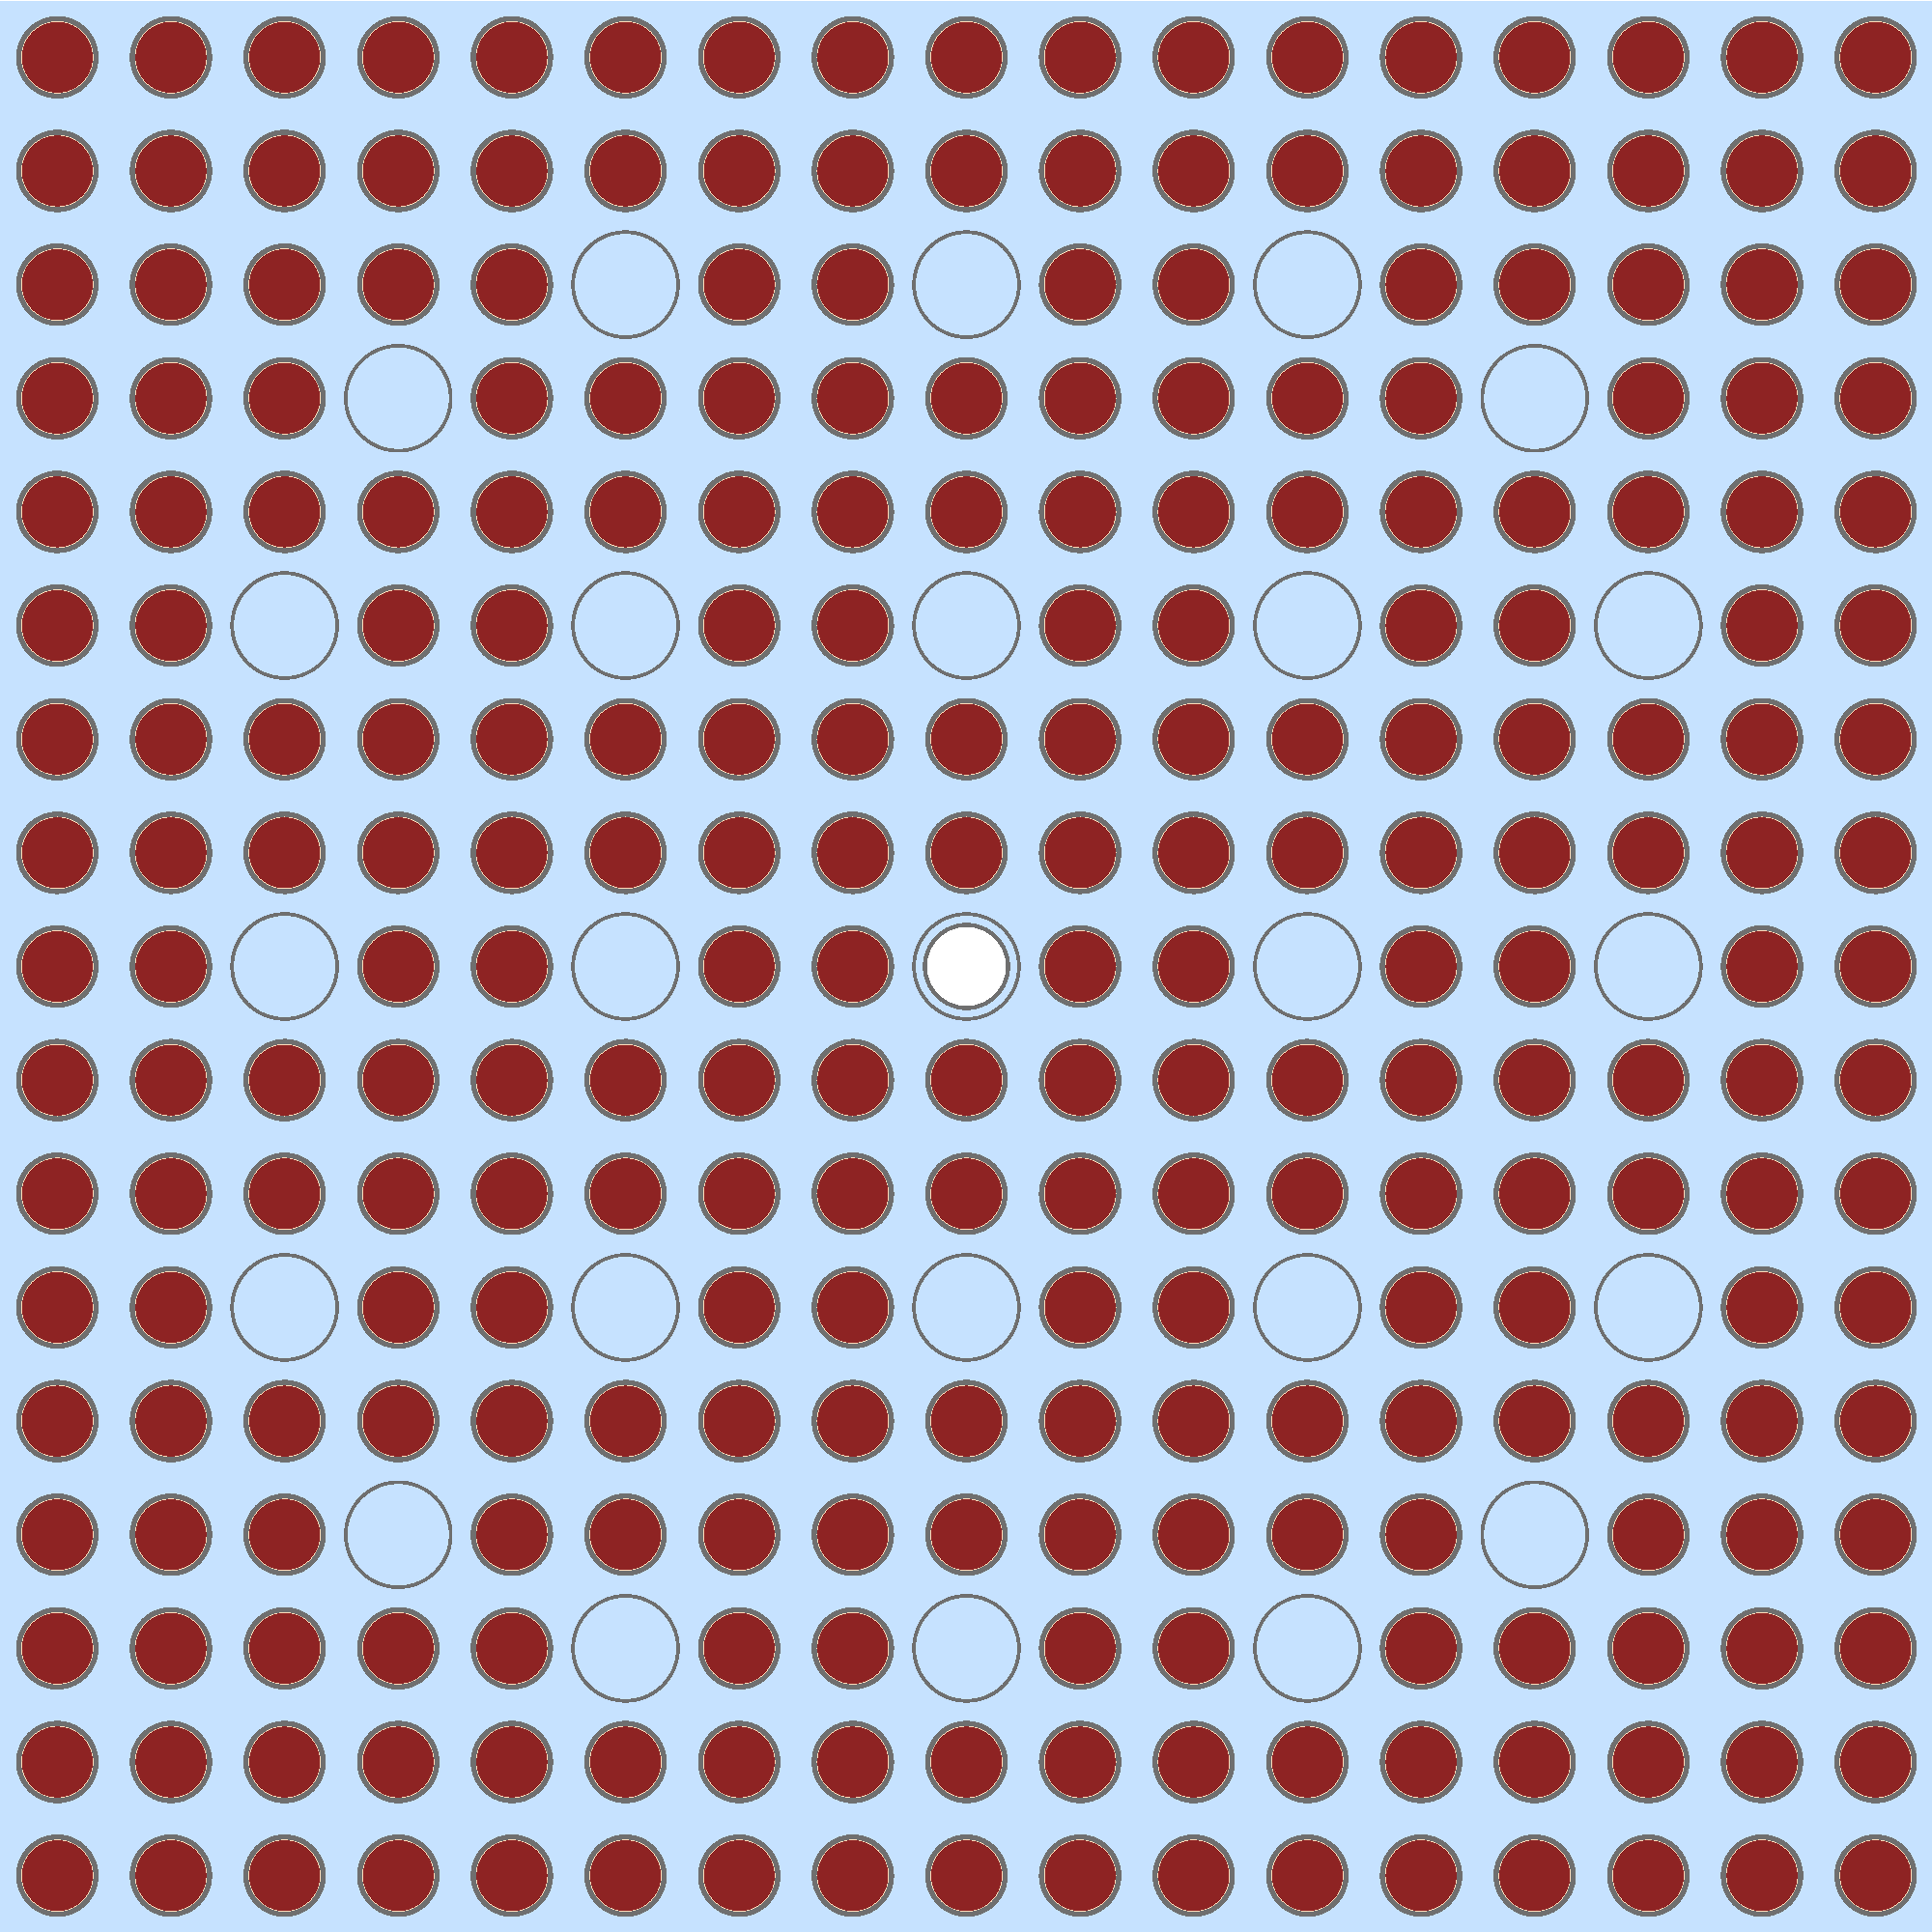
\includegraphics[width=0.8\linewidth]{figures/assembly/geometry}
  \caption{}
  \label{fig:null-assm}
\end{subfigure}
\begin{subfigure}{0.45\textwidth}
  \centering
  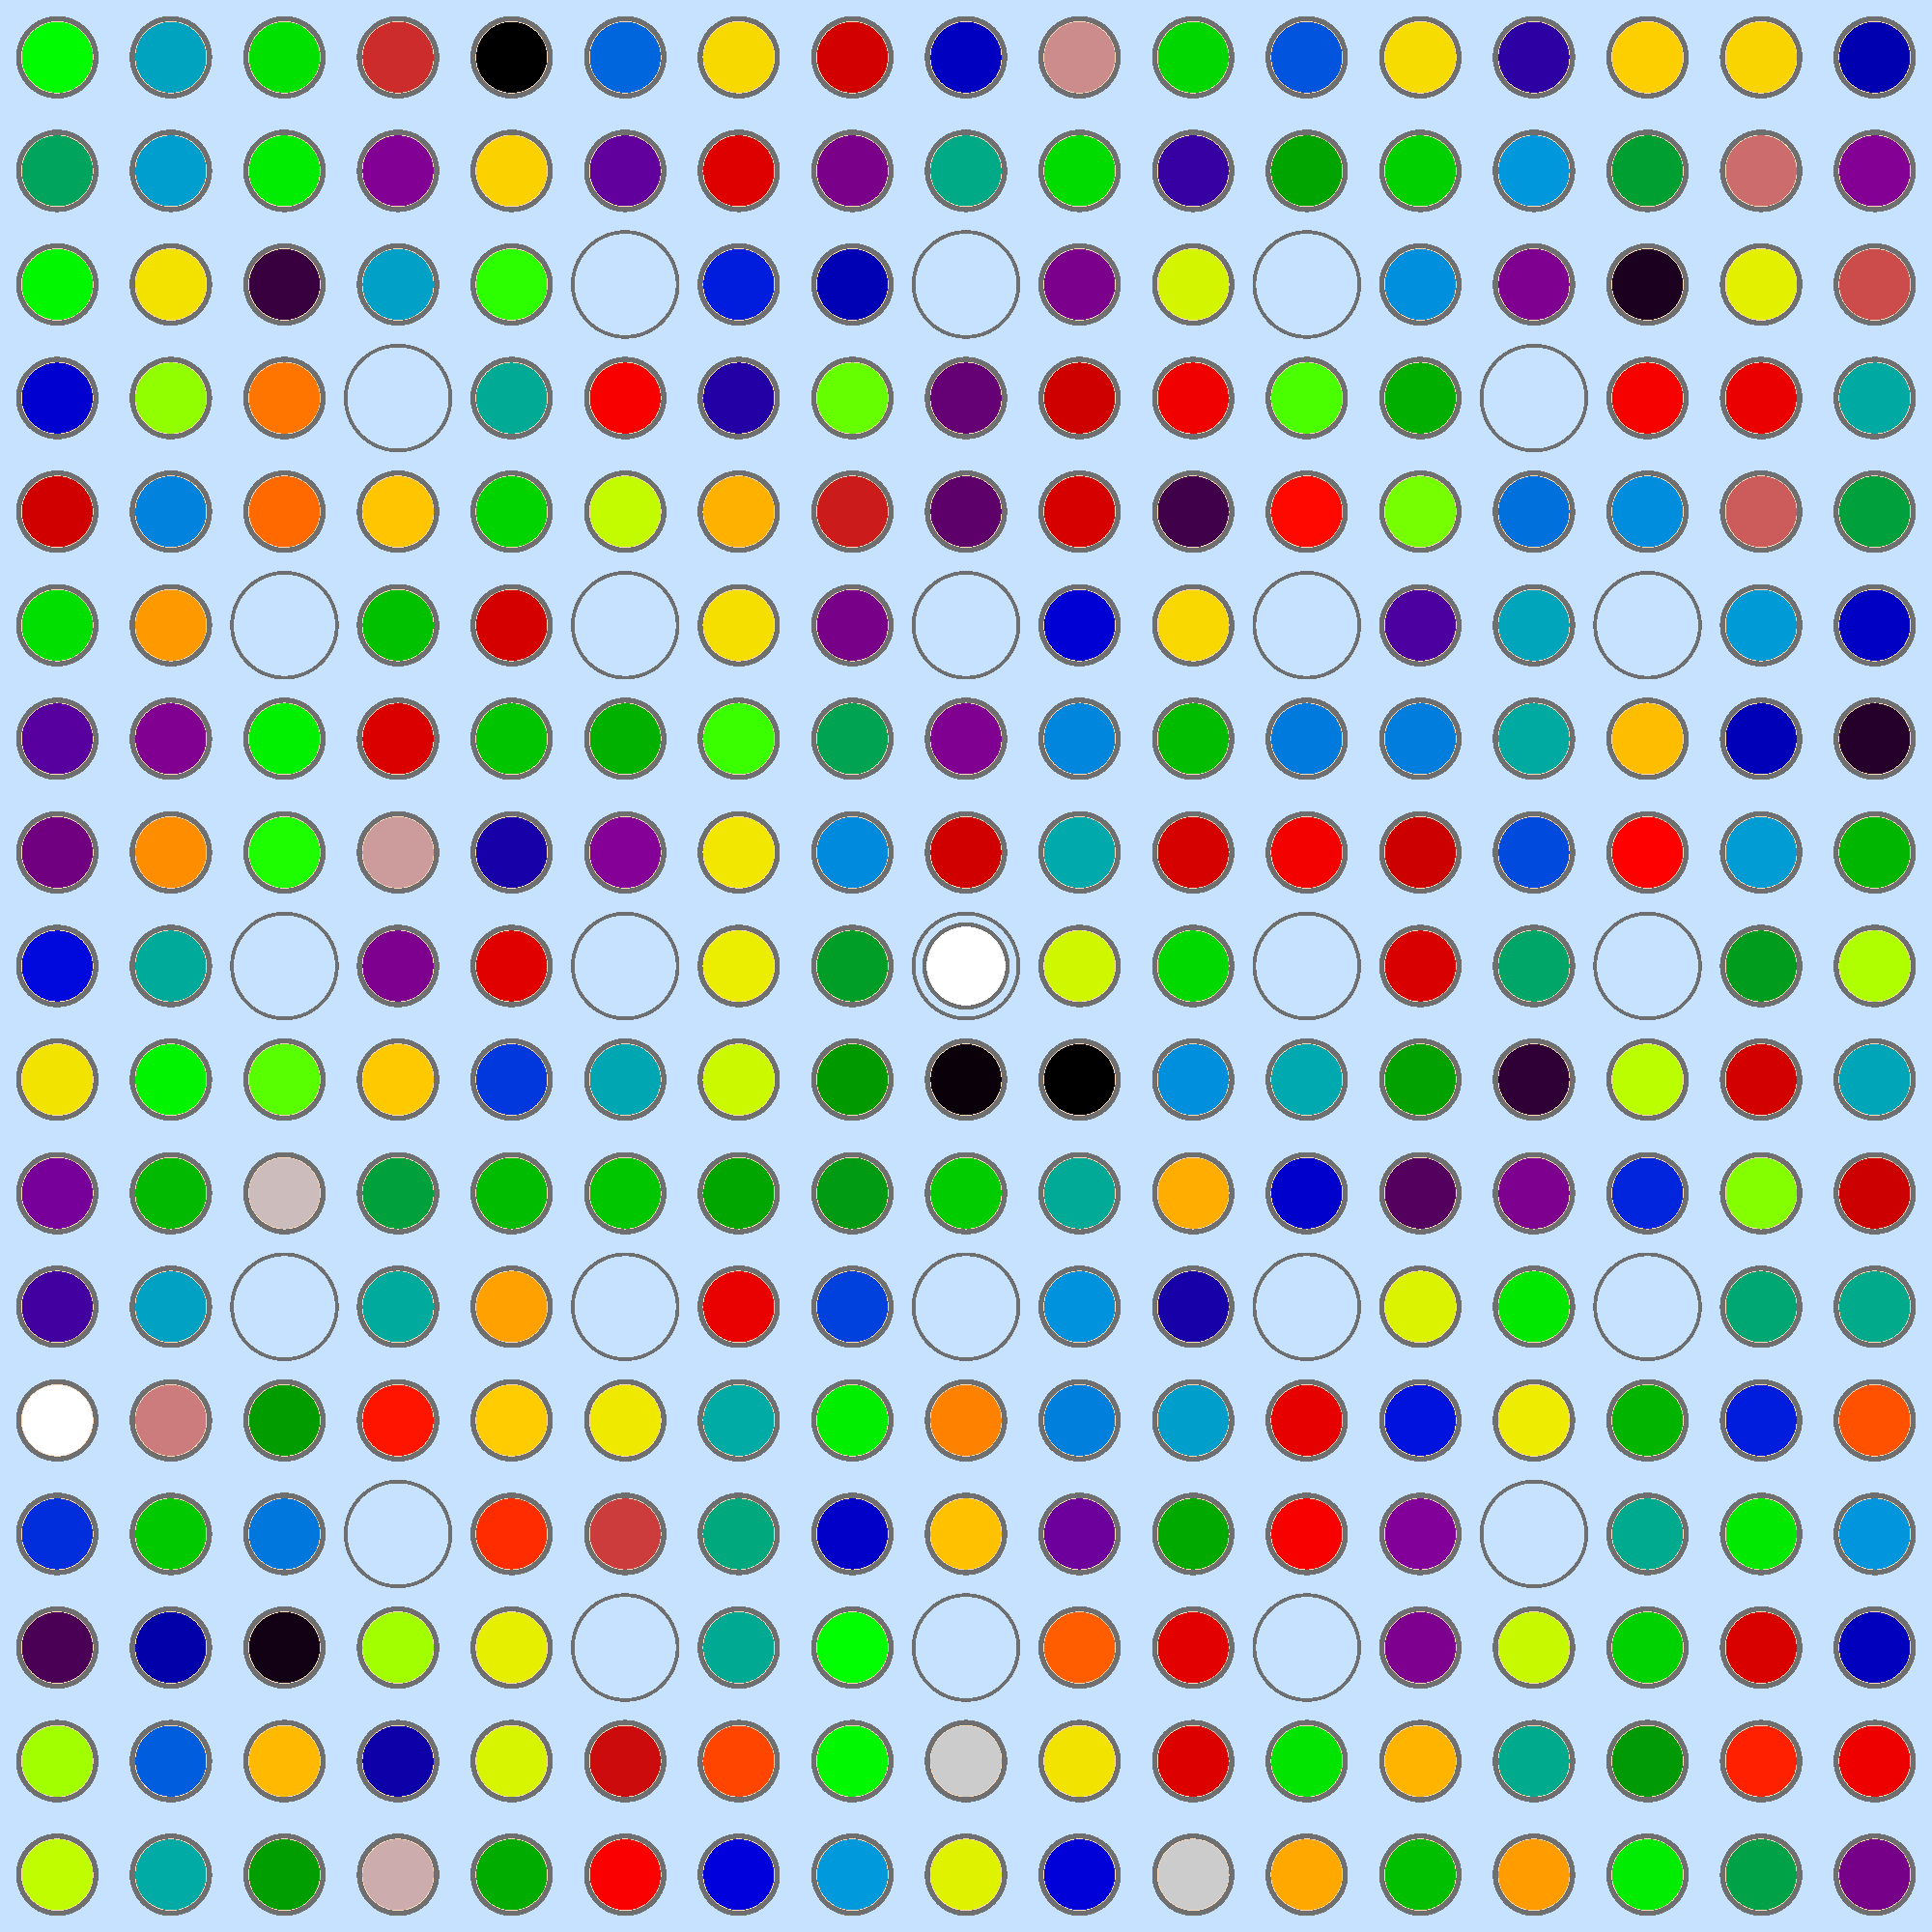
\includegraphics[width=0.8\linewidth]{figures/assembly/degenerate-materials}
  \caption{}
  \label{fig:degenerate-assm}
\end{subfigure}
\begin{subfigure}{0.45\textwidth}
  \centering
  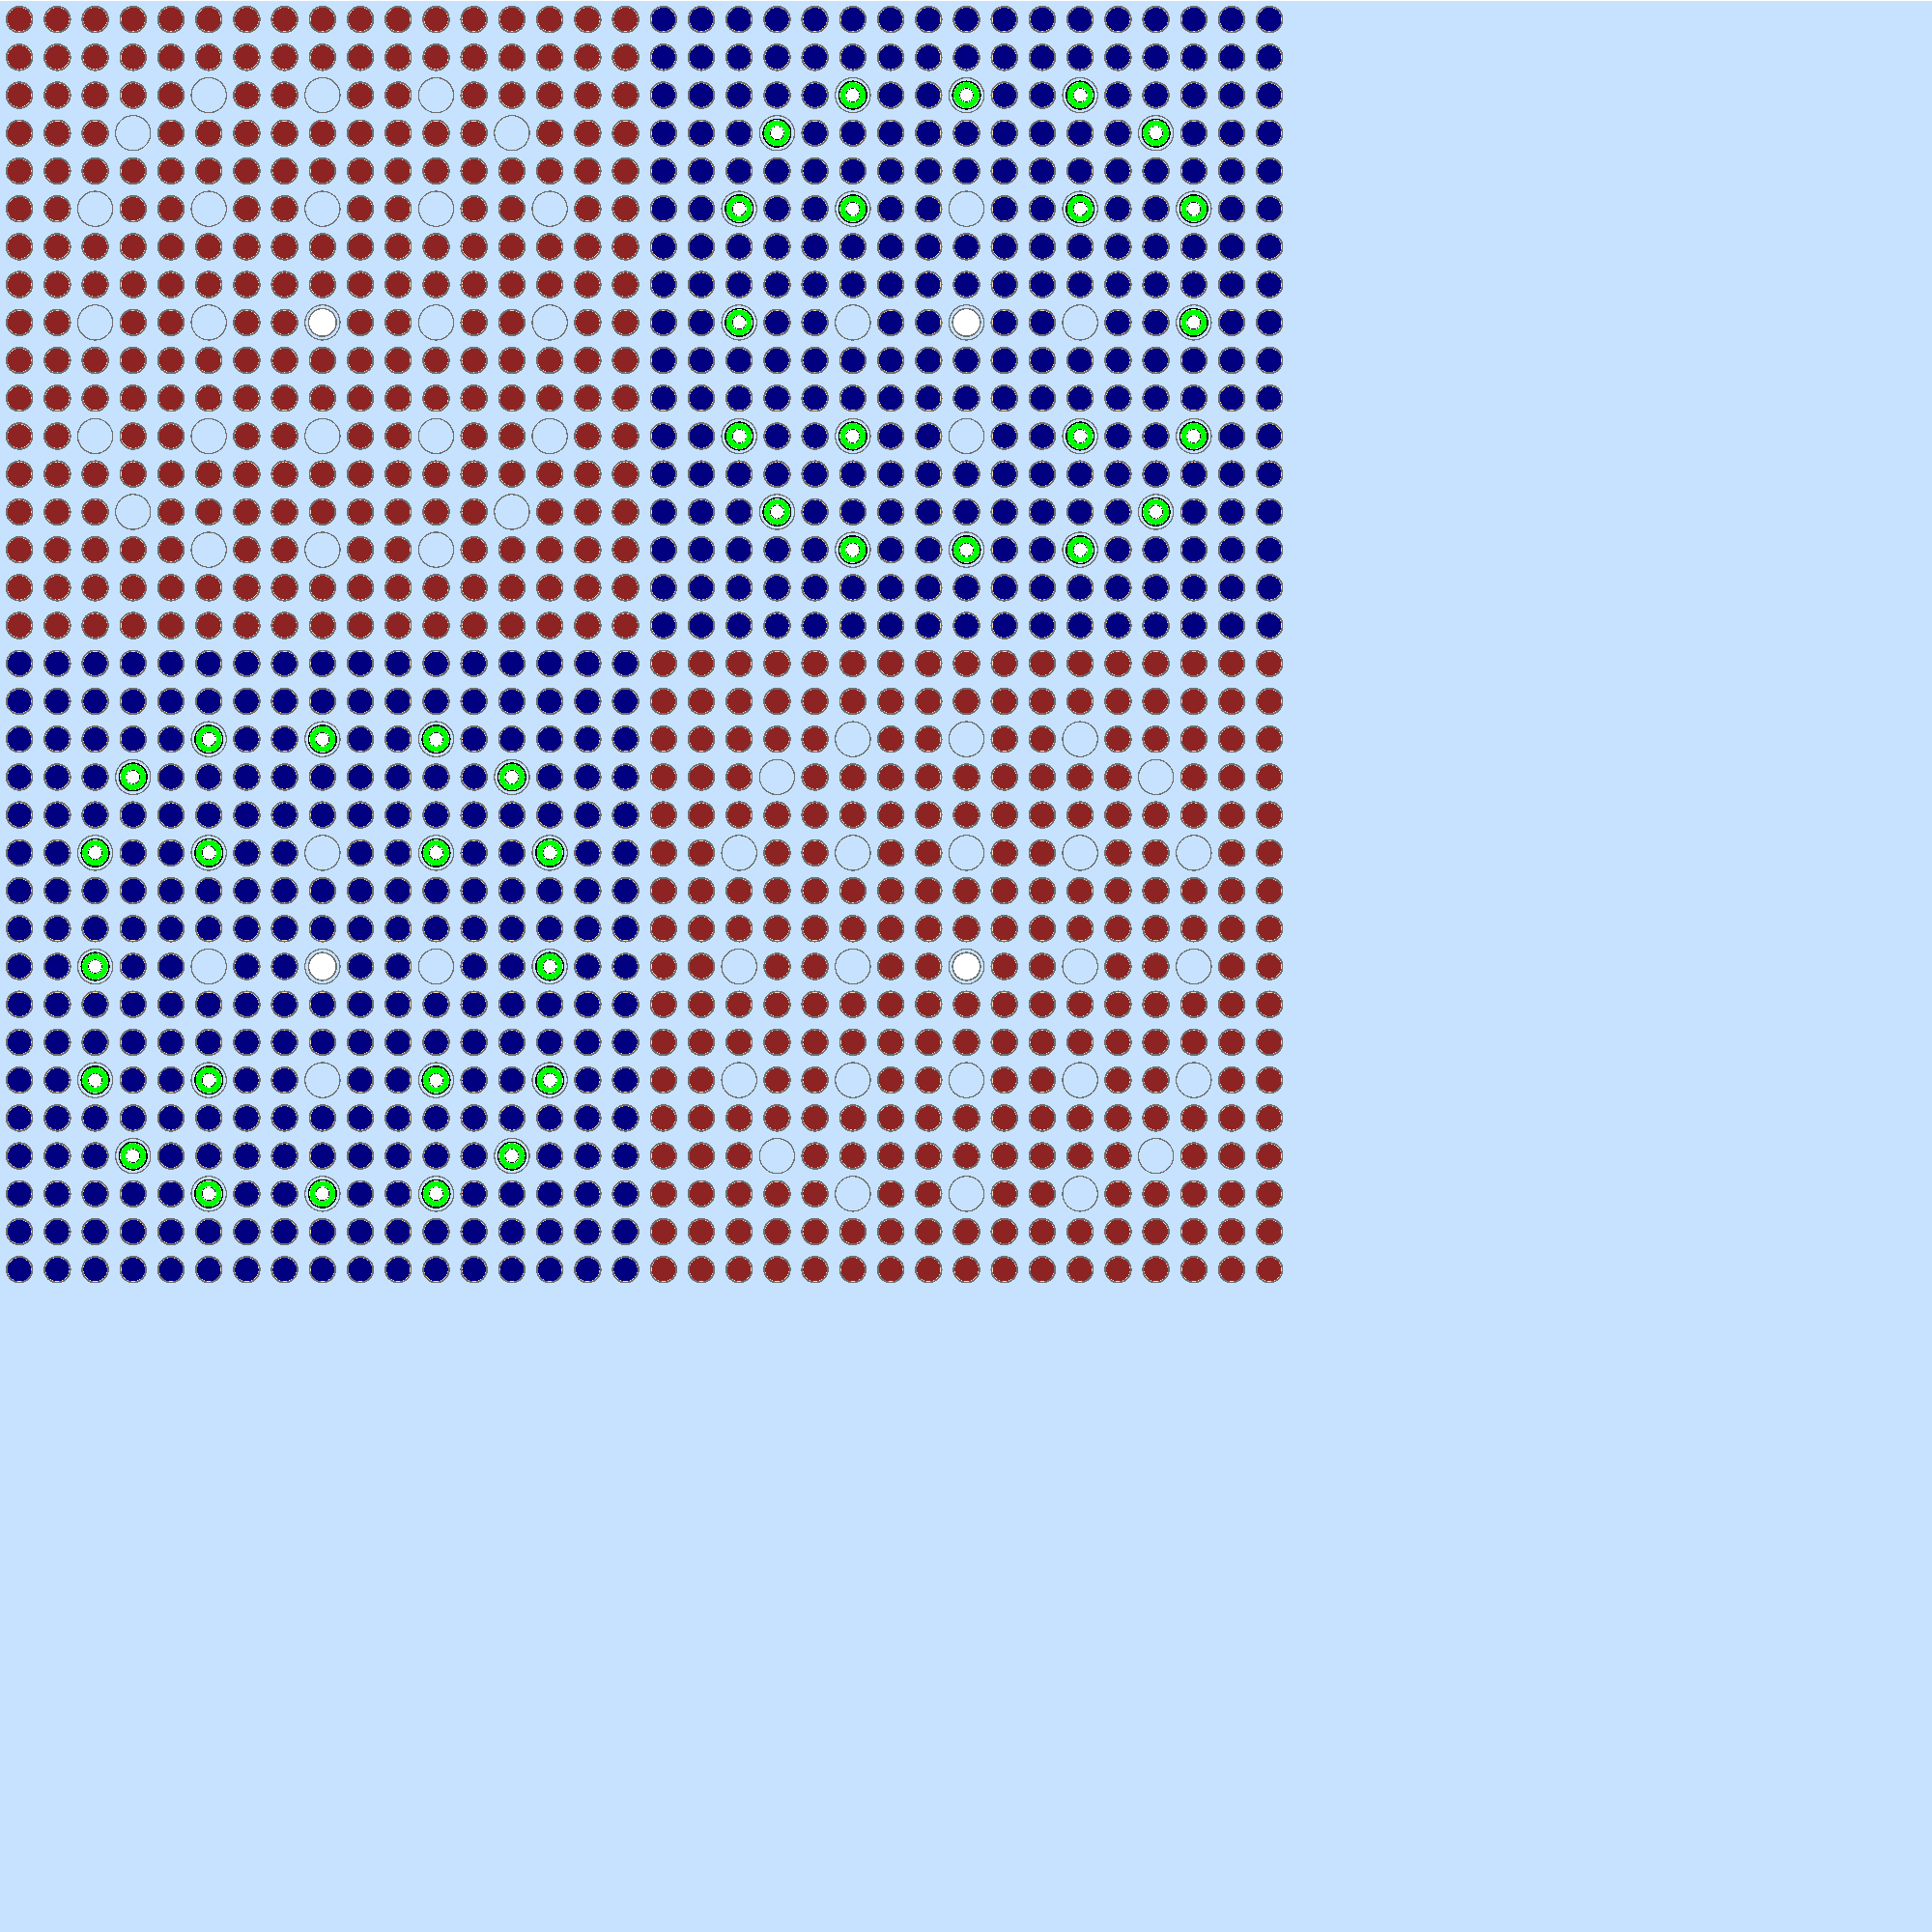
\includegraphics[width=0.8\linewidth]{figures/reflector/geometry}
  \caption{}
  \label{fig:null-reflector}
\end{subfigure}
\begin{subfigure}{0.45\textwidth}
  \centering
  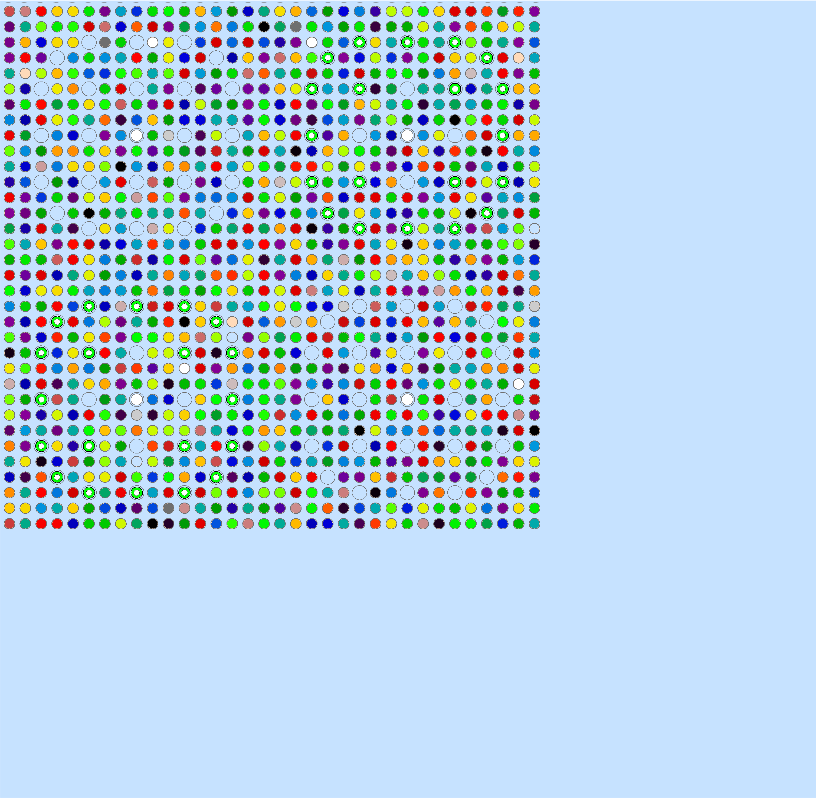
\includegraphics[width=0.8\linewidth]{figures/reflector/degenerate-materials}
  \caption{}
  \label{fig:degenerate-reflector}
\end{subfigure}
\caption{OpenMOC materials for the (a)-(b) assembly and (c)-(d) 2$\times$2 colorset models with null and degenerate homogenization, respectively.}
\label{fig:homogenization-schemes}
\end{figure*}

The \texttt{openmc.mgxs} module was used to compute 70-group MGXS with OpenMC for both the assembly and colorset benchmarks. The tallied MGXS data was condensed to coarse 2-group and 8-group structures with downstream data processing as necessary. The OpenMC simulations were performed with 1000 batches with 10$^{6}$ particle histories per batch for each benchmark. Stationarity of the fission source was obtained with 100 inactive batches for each benchmark. OpenMC's ``iso-in-lab'' feature was employed to enable consistent comparisons between OpenMC's reference results and OpenMOC's calculations with an isotropic in lab scattering source.

%%%%%%%%%%%%%%%%%%%%%%%%%%%%%%%%%%%%%%%%%%%%%%%%%%%%%%%%%%%%%%%%%%%%%%%%%%%%%%%
\subsubsection{Null Homogenization}
\label{subsubsec:homogenize-null}

The \textit{null} spatial homogenization scheme uses a single Monte Carlo calculation of the complete heterogeneous geometry to generate MGXS for each material. In this way, the null scheme fully abandons the multi-level approach used by most traditional approaches to generate MGXS. The spatially self-shielded flux is used to collapse the cross sections in each material with a unique isotopic composition. The null scheme does not account for spatial self-shielding effects experienced by different fuel pins filled by the same type of fuel, and instead averages these effects across the entire geometry. A single MGXS is employed in each instance of a material zone, such as a fuel pin replicated many times throughout a benchmark geometry.

%%%%%%%%%%%%%%%%%%%%%%%%%%%%%%%%%%%%%%%%%%%%%%%%%%%%%%%%%%%%%%%%%%%%%%%%%%%%%%%
\subsubsection{Degenerate Homogenization}
\label{subsubsec:homogenize-degenerate}

Unlike the null scheme, the \textit{degenerate} scheme accounts for the different spatial self-shielding effects experienced by each instance of each fuel pin throughout a heterogeneous geometry. Like the null scheme, a single MC calculation of the complete heterogeneous geometry is used to generate MGXS for all materials. Unlike the null scheme, the MGXS are tallied separately for each instance of fissile material zones. For example, if a heterogeneous benchmark includes $N$ fuel pins, then $N$ collections of MGXS are separately tabulated for each fuel pin instance. The degenerate scheme tallies different MGXS even if the isotopic compositions in the fuel pin instances are identical (\textit{e.g.}, fresh fuel at the beginning of life) since each instance may experience different spatial self-shielding effects and hence have different MGXS.

The degenerate scheme generates MGXS for each fuel pin instance using OpenMC's distributed cell tallies~\citep{lax2014distribcell}. The OpenCG region differentiation algorithm~\citep{boyd2015opencg} is used to build a new OpenMOC geometry with unique cells and materials for each fuel pin. The MGXS are appropriately selected from OpenMC's distributed cell tallies to populate the MGXS in the OpenMOC materials. Multi-group transport calculations with MGXS generated using null and degenerate schemes may be compared to quantify the impact of modeling spatial self-shielding effects in MGXS for fissile zones in heterogeneous geometries.